% Document Type: LaTeX
% Master File: ps3rsa.tex
% Latex Macro package for 6.001
% done by Nikhil, November, 1988
% updated by Hal, spring 1988
% updated by Arthur, fall 1989

\documentstyle[11pt]{article}

\pagestyle{myheadings}

% ALIGN EVEN- AND ODD-NUMBERED PAGES.
\evensidemargin 35pt

% NO NUMBERING ON SECTIONS
\setcounter{secnumdepth}{0}

% HORIZONTAL MARGINS
% Left margin 1 inch (0 + 1)
\setlength{\oddsidemargin}{0in}
% Text width 6.5 inch (so right margin 1 inch).
\setlength{\textwidth}{6.5in}

% ----------------
% VERTICAL MARGINS
% Top margin 0.5 inch (-0.5 + 1)
\setlength{\topmargin}{-0.5in}
% Head height 0.25 inch (where page headers go)
\setlength{\headheight}{0.25in}
% Head separation 0.25 inch (between header and top line of text)
\setlength{\headsep}{0.25in}
% Text height 8.5 inch (so bottom margin 1.5 in)
\setlength{\textheight}{8.5in}

% ----------------
% PARAGRAPH INDENTATION
\setlength{\parindent}{0in}

% SPACE BETWEEN PARAGRAPHS
\setlength{\parskip}{\medskipamount}

% ----------------
% EVALUATION SYMBOL
\newcommand{\evalsto}{$\Longrightarrow$}

% ----------------
% STRUTS
% HORIZONTAL STRUT.  One argument (width).
\newcommand{\hstrut}[1]{\hspace*{#1}}
% VERTICAL STRUT. Two arguments (offset from baseline, height).
\newcommand{\vstrut}[2]{\rule[#1]{0in}{#2}}

% ----------------
% EMPTY BOXES OF VARIOUS WIDTHS, FOR INDENTATION
\newcommand{\hm}{\hspace*{1em}}
\newcommand{\hmm}{\hspace*{2em}}
\newcommand{\hmmm}{\hspace*{3em}}
\newcommand{\hmmmm}{\hspace*{4em}}

% ----------------
% VARIOUS CONVENIENT WIDTHS RELATIVE TO THE TEXT WIDTH, FOR BOXES.
\newlength{\hlessmm}
\setlength{\hlessmm}{\textwidth}
\addtolength{\hlessmm}{-2em}

\newlength{\hlessmmmm}
\setlength{\hlessmmmm}{\textwidth}
\addtolength{\hlessmmmm}{-4em}

% ----------------
% ``TIGHTLIST'' ENVIRONMENT (no para space between items, small indent)
\newenvironment{tightlist}%
{\begin{list}{$\bullet$}{%
    \setlength{\topsep}{0in}
    \setlength{\partopsep}{0in}
    \setlength{\itemsep}{0in}
    \setlength{\parsep}{0in}
    \setlength{\leftmargin}{1.5em}
    \setlength{\rightmargin}{0in}
    \setlength{\itemindent}{0in}
}
}%
{\end{list}
}

% ----------------
% CODE FONT (e.g. {\cf x := 0}).
\newcommand{\cf}{\footnotesize\tt}

% ----------------
% INSTRUCTION POINTER
\newcommand{\IP}{$\bullet$}
\newcommand{\goesto}{$\longrightarrow$}

% ----------------------------------------------------------------
% LISP CODE DISPLAYS.
% Lisp code displays are enclosed between \bid and \eid.
% Most characters are taken verbatim, in typewriter font,
% Except:
%  Commands are still available (beginning with \)
%  Math mode is still available (beginning with $)

\outer\def\beginlisp{%
  \begin{minipage}[t]{\linewidth}
  \begin{list}{$\bullet$}{%
    \setlength{\topsep}{0in}
    \setlength{\partopsep}{0in}
    \setlength{\itemsep}{0in}
    \setlength{\parsep}{0in}
    \setlength{\leftmargin}{1.5em}
    \setlength{\rightmargin}{0in}
    \setlength{\itemindent}{0in}
  }\item[]
  \obeyspaces
  \obeylines \footnotesize\tt}

\outer\def\endlisp{%
  \end{list}
  \end{minipage}
  }

{\obeyspaces\gdef {\ }}

% ----------------
% ILLUSTRATIONS
% This command should specify a NEWT directory for ps files for illustrations.
\def\psfileprefix{/usr/nikhil/parle/}
\def\illustration#1#2{
\vbox to #2{\vfill\special{psfile=\psfileprefix#1.ps hoffset=-72 voffset=-45}}} 

% \illuswidth is used to set up boxes around illustrations.
\newlength{\illuswidth}
\setlength{\illuswidth}{\textwidth}
\addtolength{\illuswidth}{-7pt}

% ----------------------------------------------------------------
% SCHEME CLOSURES AND PROCEDURES

% CLOSURES: TWO CIRCLES BESIDE EACH OTHER; LEFT ONE POINTS DOWN TO CODE (arg 1)
% RIGHT ONE POINTS RIGHT TO ENVIRONMENT (arg 2)
\newcommand{\closure}[2]{%
\begin{tabular}[t]{l}
\raisebox{-1.5ex}{%
  \setlength{\unitlength}{0.2ex}
  \begin{picture}(25,15)(0,-7)
   \put( 5,5){\circle{10}}
   \put( 5,5){\circle*{1}}
   \put( 5,5){\vector(0,-1){10}}
   \put(15,5){\circle{10}}
   \put(15,5){\circle*{1}}
   \put(15,5){\vector(1,0){12}}
  \end{picture}}
  \fbox{\footnotesize #2} \\
%
\hspace*{0.8ex} \fbox{\footnotesize #1}
\end{tabular}
}

% PROCEDURES: BOX CONTAINING PARAMETERS (arg 1) AND BODY (arg 2)
\newcommand{\proc}[2]{%
\begin{tabular}{l}
params: #1 \\
body: #2 \\
\end{tabular}
}

% PROBLEM SET HEADER -- args are semester and problem set or solution
% example: \psetheader{Spring Semester, 1989}{Problem set 1}
\newcommand{\psetheader}[2]{%
\markright{6.001, #1---#2}
\begin{center}
MASSACHVSETTS INSTITVTE OF TECHNOLOGY \\
Department of Electrical Engineering and Computer Science \\
6.001---Structure and Interpretation of Computer Programs \\
#1 \\
\medskip
{\bf #2}
\end{center}
}

% PROBLEM HEADER
\newcommand{\problem}[1]{{\bf #1}}

% KEYS
\newcommand{\key}[1]{\fbox{{\sc #1}}}
\newcommand{\ctrl}{\key{ctrl}--}
\newcommand{\shift}{\key{shift}--}
\newcommand{\run}{\key{run} \ }
\newcommand{\runkey}[1]{\run \key{#1}}
\newcommand{\extend}{\key{extend} \ }
\newcommand{\kkey}[1]{\key{k$_{#1}$}}

%% Examples of keys
%% \key{abort}
%% \ctrl\key{g}
%% \extend\key{logout}
%% \kkey{1}
%% \shift\kkey{1}

% ----------------------------------------------------------------
% HERE BEGINS THE DOCUMENT
% start with \begin{document}


\def\fbox#1{%
  \vtop{\vbox{\hrule%
     \hbox{\vrule\kern3pt%
 \vtop{\vbox{\kern3pt#1}\kern3pt}%
 \kern3pt\vrule}}%
 \hrule}}
\usepackage{../epsfig}
\begin{document}

%%%%%%%%%%%%%%%%%%%%%%%%%%%%%%%%%%%%%%%%%%%%%%%%%%%%%%%%%%%%%%%%%%%%%%%%%%%%%%%

\psetheader{Sample Problem Set}{RSA Encryption}

%%%%%%%%%%%%%%%%%%%%%%%%%%%%%%%%%%%%%%%%%%%%%%%%%%%%%%%%%%%%%%%%%%%%%%%%%%%%%%%

\begin{center}
{\bf Public-Key Encryption and Digital Signatures }
\end{center}


\medskip

The ideas of {\it public-key encryption} and {\it digital signatures}
were discovered only in 1976.  But they already play a fundamental
role as a way to achieve private communication in a world that relies
increasingly upon digital information.  Interestingly, the fact that
there are fast algorithms for exponentiation and for testing prime
numbers (sections 1.2.4--1.2.6 of the text) lies at the root of
RSA---the most popular method for implementing public-key encryption.
In this problem set you will implement a version of the RSA system.
By doing so, you will gain experience with some algorithms that
although simple, have immense practical importance.\footnote{This
problem set was designed in 1987 by Ruth Shyu and Eric Grimson and
revised in 1992 by David LaMacchia and Hal Abelson.} Section 1 of this
handout desccribes how the system works.  Section 2 contains exercises
that you should be prepared to discuss in tutorial.  Section 3
contains background for the lab assigment, and section 4 is the actual
lab assignment.


\section{1. The RSA System}

People have been using secret codes for thousands of years; for this
reason it is surprising that in 1976, Whitfield Diffie and Martin Hellman
at Stanford University discovered a major new conceptual approach to
encryption and decryption; {\it public-key cryptography}.\footnote{W.
Diffie and M. Hellman, ``New directions in cryptography,'' {\it IEEE
Transactions on Information Theory}, IT-22:6, 1976, pp 644--654.}

Cryptography systems are typically based on the notion of using {\it
keys} for encryption and decryption.  An {\it encryption key}
specifies the method for converting the original message into an
encoded form.  A corresponding {\it decryption key} describes how to
undo the encoding.  In traditional cryptographic systems, the
decryption key is identical to the encryption key, or can be readily
derived from it.  As a consequence, if you know how to {\it encrypt}
messages with a particular key then you can easily {\it decrypt}
messages that were encrypted with that key.

Diffie and Hellman's insight was to realize that there are
cryptographic systems for which knowing the encryption key gives no
help in decrypting messages; that is, for which there is no practical
way to derive the decryption key from the encryption key.  This is of
immense practical importance.  In traditional cryptographic systems,
someone can send you coded messages only if the two of you share a
secret key.  Since anyone who learns that key would be able to decrypt
the messages, keys must be carefully guarded and transmitted only
under tight security.  In Diffie and Hellman's system, you can tell
your {\it encryption} key to anyone who wants to send you messages,
and not worry about key security at all.  For even if everyone in the
world knew your encryption key, no one could decrypt messages sent to
you without knowing your {\it decryption key}, which you keep private
to yourself.  Diffie and Hellman called such a system a {\it
public-key} cryptography system.

A few months after Diffie and Hellman announced their idea, Ronald
Rivest, Adi Shamir, and Leonard Adelman at MIT discovered a workable
method for implementing it.  This {\it RSA cryptography system} has
remained the most popular technique for public-key cryptography.


\subsection{The theory behind RSA}

RSA uses integers to represent groups of characters\footnote{For
example, the ASCII standard representation of a character is a 7-bit
integer.  In this problem set we will represent a block of four
characters as a 28-bit integer ($0 \leq s < 2^{28}$) by concatenating
the ASCII codes of the four characters.} and uses special
functions that transform integers to integers.

In the RSA scheme, you select two large prime numbers, $p$ and $q$.
You then define
\begin{eqnarray}
n&=& pq\\
m&=&(p - 1)(q - 1).
\end{eqnarray}
You also select a number $e$, such that $\gcd(e,m)=1$.  Your {\it
public key}, which you can advertise to the world, is the pair of
numbers $n$ and $e$.  Anyone who wants to send you a message $s$
(represented by an integer) encrypts it using the following {\it RSA
transformation} defined by $n$ and $e$:

\smallskip
\centerline{encrypted message = $s$ to the power of $e$, modulo $n$}
or
\[S = (s^e) \bmod n.\]

If you receive an encrypted message $S$, you decrypt it by performing
another RSA transformation with $n$ and a special number $d$:

\smallskip \centerline{$s^\prime$ = encrypted message to the power of
$d$, modulo $n$} or \[s^\prime = (S^d) \bmod n.\]

The number $d$ is chosen to have the property that $s = s^\prime$ for
every message $s$,\footnote{Actually, this is true only if
$\gcd(s,n)=1$.  If $n$ is the product of two large primes, then almost
all messages $s<n$ will satisfy this.} namely,

\[s = (s^e)^d \bmod n.\]

It can be shown that the number $d$ that has this property is the one
for which
\begin{equation}
de=1 \bmod m
\end{equation}
that is, for which $d$ is the {\it multiplicative inverse} of $e$
modulo $m$.\footnote{This is a basic result in number theory , we'll
just ask you to take it on faith.} It turns out that it is easy to compute $d$
efficiently if you know $e$ and $m=(p-1)(q-1)$.

Thus, to generate a pair of RSA keys, you choose prime numbers $p$
and $q$, compute $n=pq$, choose $e$, and use this to compute $d$.
You publish the pair $n$ and $e$ as your public key, but keep $d$
secret to yourself.  People send you encrypted messages using the
pair $(n,e)$.  You decrypt these messages using the pair $(n,d)$.

The security of the RSA system is based on the fact that even if
someone knows $e$ and $n$, the most efficient way known for them to
decrypt a message is to factor $n$ to find $p$ and $q$, then use
these to compute $m$, then use $e$ and $m$ to compute $d$.

That is to say, cracking an RSA code is, as far as anyone knows, as
difficult a computational problem as factoring $n$ into its prime
factors $p$ times $q$.  And although there has been a tremendous
amount of research on factoring, factoring arbitrary large numbers is
not a computationally feasible task.  For example, factoring $n=pq$
where $p$ and $q$ are each 200-digit primes, even with the today's
best factoring algorithms, would require running for more than 100
years on today's fastest supercomputers.\footnote{No one has actually
proved that cracking an RSA code is as difficult a problem as
factoring, but no other method for cracking these codes has been
discovered.  In addition, some computer scientists believe that it
may be possible to prove that there can be no fast (e.g., logarithmic
time) algorithms for factoring.  Given the popularity of RSA, the
discovery of such an algorithm would result in a massive security
breakdown for banks, businesses, and other organizations that use
RSA.}


\subsection{Digital signatures; Encrypting and signing}

In their 1976 paper, Diffie and Hellman suggested applying public-key
encryption to solving another important problem of secure
communication.  The problem is this: suppose you want to send a
message by electronic mail.  How can people who receive the message be
sure that it really comes from you---that it is not a forgery?  What
is required is some scheme for marking a message in a way that cannot
be forged.  Such a mark is called a {\it digital signature}.

Diffie and Hellman's suggestion was to proceed as follows: take the
message and apply a publicly agreed upon {\it compression function}
(also called a {\it hash function}) that transforms the message to a
single, relatively small number.  In general, there will be many
messages that produce the same hash value.  Now transform the hash
value using your private key.  The transformed hash value is your
digital signature, which you transmit along with the message.  Anyone
who receives a message can authenticate the signature by transforming
it using your {\it public key} and checking that this gives the same
result as applying the compression function to the message.

The reason this scheme works is that anyone who wants to forge a
message claiming to be from you must produce a number that, when
transformed by your public key, matches the hash value.  Anyone can
compute the hash value, since the compression function is assumed to
be public.  But since you are assumed to be the only one who knows
your private key, only you can produce the number which is
transformed to the hash value by your public key.  Trying to forge a
digital signature is essentially the same task as trying to crack a
public-key encrypted message.

An even cuter idea works as follows: Suppose Barbara wants to send
George a signed message that only George will be able to read.  She
encrypts the message using George's public key.  Then she signs the
encrypted result using her own private key.  When George receives a
message that is supposed to be from Barbara, he first uses Barbara's
public key to authenticate the signature, then decrypts the message
using his own private key.  Figure~\ref{digital-signature} gives an
overview of the method.

\begin{figure}
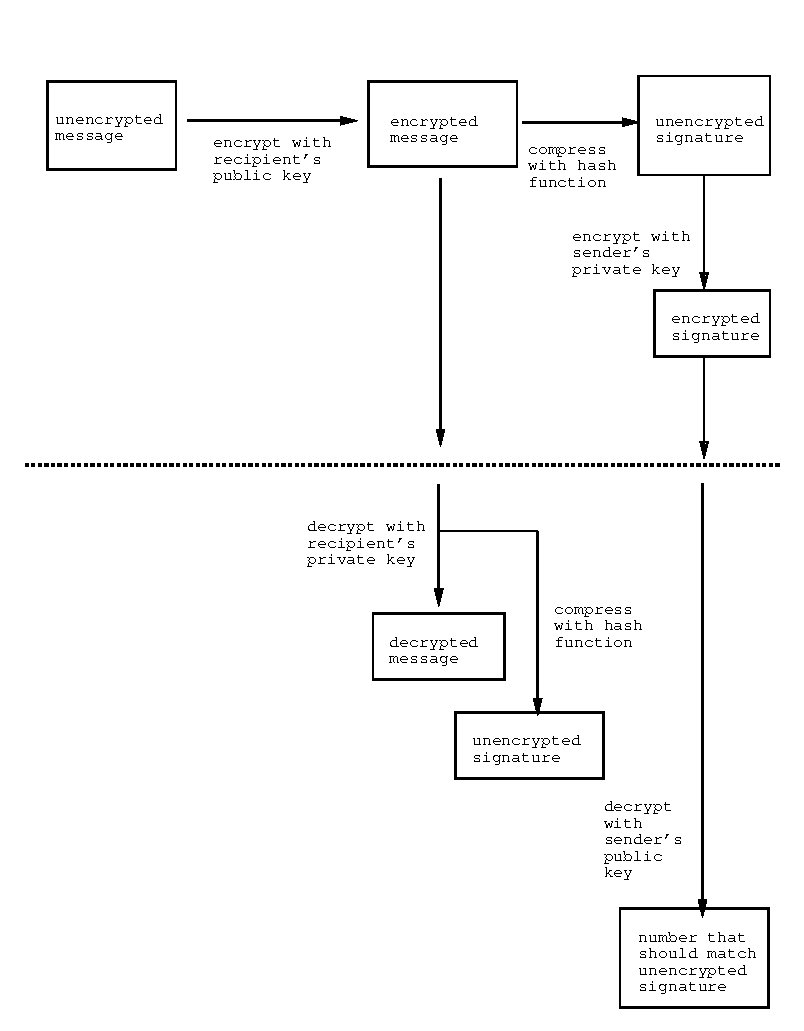
\epsfig{file=./figure1.ps}
\caption {Encryption with digital signature.}
\label{digital-signature}
\end{figure}

Notice what this accomplishes: George can be sure that only someone
with Barbara's private key could have sent the message.  Barbara can
be sure that only someone with George's private key can read the
message.  This is accomplished without exchanging any secret
information between George and Barbara.  It's this capacity for
achieving secure communication without having to worry about
exchanging secret keys that makes public-key cryptography such an
important technique.


\subsection{Implementing RSA}

The primary thing we need in order to implement RSA is the fast
exponentiation algorithm from section 1.2.6 of the text:

\beginlisp
(define (expmod b e m)
  (cond ((zero? e) 1)
        ((even? e)
         (remainder (square (expmod b (/ e 2) m)) m))
        (else (remainder (* b (expmod b (- e 1) m)) m))))
\endlisp

\noindent
We'll assume that an RSA key is represented as a pair---modulus and exponent:

\beginlisp
(define make-key cons)
(define key-modulus car)
(define key-exponent cdr)
\endlisp

\noindent
The basic RSA transformation is then

\beginlisp
(define (RSA-transform number key)
  (expmod number (key-exponent key) (key-modulus key)))
\endlisp

\subsubsection{Generating prime numbers}

To generate RSA keys, we first of all need a way to generate primes.
The most straightforward way is to pick a random number in some
desired range and start testing successive numbers from there until we
find a prime.  The following procedure starts searching at a randomly
chosen integer between {\tt start} and ${\tt start}+{\tt range}$:

\beginlisp
(define (choose-prime smallest range)
  (let ((start (+ smallest (choose-random range))))
    (search-for-prime (if (even? start) (+ start 1) start))))
\null
(define (search-for-prime guess)
  (if (fast-prime? guess 2)
      guess
      (search-for-prime (+ guess 2))))
\null
(define choose-random
  ;; restriction of Scheme RANDOM primitive
  (let ((max-random-number (expt 10 18)))
    (lambda (n)
      (random (floor->exact (min n max-random-number))))))
\endlisp

The test for primality is the Fermat test, described in section 1.2.6:

\beginlisp
(define (fermat-test n)
    (let ((a (choose-random n)))
      (= (expmod a n n) a)))
\null
(define (fast-prime? n times)
    (cond ((zero? times) true)
          ((fermat-test n) (fast-prime? n (- times 1)))
          (else false)))
\endlisp


\subsubsection{Generating RSA key pairs}

Now we can generate a public RSA key and matching private key.  We'll
represent these as a pair:

\beginlisp
(define make-key-pair cons)
(define key-pair-public car)
(define key-pair-private cdr)
\endlisp

The following procedure generates an RSA key pair.  It picks primes
$p$ and $q$ that are in the range from $2^{14}$ to $2^{15}$ so that
$n=pq$ will be in the range $2^{28}$ to $2^{30}$, which is large
enough to encode four characters per number.\footnote{We're using
such small values of $n$ for this problem set because we want you to
play around with cracking an RSA system.  By starting with larger
random numbers, you can use the same method to produce a system that
really is secure.}  After picking the primes, it computes $n$ and $m$
according to equations (1) and (2).  It then chooses an
exponent $e$ and finds a number $d$ that satisfies equation (3).

\beginlisp
(define (generate-RSA-key-pair)
  (let ((size (expt 2 14)))
    (let ((p (choose-prime size size))
          (q (choose-prime size size)))
      (if (= p q)                 ;check that we haven't chosen the same prime twice
          (generate-RSA-key-pair) ;(VERY unlikely)
          (let ((n (* p q))
                (m (* (- p 1) (- q 1))))
            (let ((e (select-exponent m)))
              (let ((d (invert-modulo e m)))
                (make-key-pair (make-key n e) (make-key n d)))))))))
\endlisp

The exponent $e$ can be any random number $0<e<m$ with $\gcd(e,m)=1$.
The {\tt gcd} procedure is given in section 1.2.5 of the notes, but is
actually a Scheme primitive.

\beginlisp
(define (select-exponent m)
  (let ((try (choose-random m)))
    (if (= (gcd try m) 1)       ;if gcd is not 1, then try again
        try
        (select-exponent m))))
\endlisp

\subsubsection{Computing the multiplicative inverse}

The number $d$ required for the RSA key must satisfy
\[de=1 \bmod m\]
Using the definition of equality modulo $m$, this means that $d$ must
satisfy
\[km + de=1\]
where $k$ is a (negative) integer.  One can show that a solution to
this equation exists if and only if $\gcd(e,m)=1$.  The following
procedure generates the required value of $d$, assuming that we have
another procedure available which, given two integers $a$ and $b$,
returns a pair of integers $(x,y)$ such that $ax+by=1$.\footnote{The
Scheme primitive {\tt modulo}, which we use to insure a positive
result, is the same as {\tt remainder}, except on negative arguments:
{\tt (remainder -12 7)} is $-5$, while {\tt (modulo -12 7)} is 2.  In
general, {\tt (modulo a b)} always has the same sign as {\tt b}, while
{\tt (remainder a b)} always has the same sign as {\tt a}.}

\beginlisp
(define (invert-modulo e m)
  (if (= (gcd e m) 1)
      (let ((y (cdr (solve-ax+by=1 m e))))
        (modulo y m))   ;take y modulo m, in case y was negative
      (error "gcd not 1" e m)))
\endlisp

Solving $ax+by=1$ can be accomplished by a nice recursive trick that
is closely related to the recursive GCD algorithm in section
1.2.5 of the text.  Let $q$ be the quotient of $a$ by $b$, and let
$r$ be the remainder of $a$ by $b$, so that
\[a=bq+r\]
Now (recursively) solve the equation
\[b\bar{x}+r\bar{y}=1\]
and use $\bar{x}$ and $\bar{y}$ to generate $x$ and $y$.  We'll leave
to you the details of how to write the actual procedure.  (Ask in
recitation.)

\subsubsection{Encrypting and decrypting messages}

Finally, to use RSA, we need a way to transform between strings of
characters and numbers.  The code for this problem set includes
procedures {\tt string->intlist} and {\tt intlist->string} that
convert between character strings and lists of integers.  Each integer
(between 0 and $2^{28}$) encodes 4 successive characters from the
message.  If the number of characters is not a multiple of 4, the
message is padded by appending spaces:

\beginlisp
(string->intlist "This is a string.")
;Value: (242906196 69006496 245157985 217822450 67637294)
\null
(intlist->string '(242906196 69006496 245157985 217822450 67637294))
;Value: "This is a string.   "
\endlisp

\noindent
The code for these two procedures is included with the problem set
code, but you are not responsible for it.  You may want to look at it
if you are interested in how character strings can be manipulated in
Scheme.

To encrypt a message, we transform the message into a list of numbers
and convert the list of numbers using the RSA process together with
one key in the key pair.

\beginlisp
(define (RSA-encrypt string key1)
  (RSA-convert-list (string->intlist string) key1))
\endlisp

\noindent

You might guess that the right way to encode the list of numbers would
be to encode each number in the list separately.  But this doesn't
work well.  (See exercise 5 below.)  Instead, we encrypt the
first number, subrract that from the second number (modulo $n$) and
encrypt the result, add that to the next number and encrypt the
result, and so on, so that each number in the resulting encrypted list
will depend upon all the previous numbers:

\beginlisp
(define (RSA-convert-list intlist key)
  (let ((n (key-modulus key)))
    (define (convert l sum)
      (if (null? l)
          '()
          (let ((x (RSA-transform (modulo (- (car l) sum) n)
                                  key)))
            (cons x (convert (cdr l) x)))))
    (convert intlist 0)))
\endlisp

We'll leave it to you to implement the analogous {\tt
RSA-unconvert-list} procedure that undoes this transformation using
the other key in the key pair.  Then
we have

\beginlisp
(define (RSA-decrypt intlist key2)
  (intlist->string (RSA-unconvert-list intlist key2)))
\endlisp


Finally, to generate digital signatures for encrypted messages, we
need a standard compression function.  In this problem set, we'll
simply add the integers modulo $2^{28}$.\footnote{In practice, people
use more complicated compression schemes than this.  You might want to
think about why.}

\beginlisp
(define (compress intlist)
  (define (add-loop l)
    (if (null? l)
        0
        (+ (car l) (add-loop (cdr l)))))
  (modulo (add-loop intlist) (expt 2 28)))
\endlisp

\pagebreak

%==========================================================================
\section{2. Exercises}

\paragraph{Exercise 1:}
What is the difference between the following two ways of defining {\tt choose-prime}?\\
\beginlisp
(define (choose-prime smallest range)
  (search-for-prime (+ smallest (choose-random range))))
\null
(define choose-prime
  (lambda (smallest range)
    (search-for-prime (+ smallest (choose-random range)))))
\endlisp

\paragraph{Exercise 2:}
Using the representation for key pairs described above, draw the
box-and-pointer structure for a typical value returned by {\tt
generate-RSA-key-pair}.

\paragraph{Exercise 3:}
The method of sending secure signed
messages outlined above says that the sender should first encrypt the
message and then sign the result.  Would it be better to first sign
and then encrypt?

\paragraph{Exercise 4:}

The procedure {\tt RSA-encrypt} would be much simpler if we were
to encrypt each number in the list separately:

\beginlisp
(define (RSA-encrypt intlist key1)
    (map (lambda (int) (RSA-transform int key1))
         intlist))
\endlisp

\noindent
What would be the analogous {\tt RSA-decrypt} procedure?  Why is this
simple scheme inadequate for secure encryption?

\vfill
\newpage
%==========================================================================
\section{3. Background for a Programming Assignment}

\rule{6.5 in}{0.5 pt}

{\sf
\centerline{\Large\sf Ministry of Information}

To:   Ross (the Boss) \\
From: Rupert

So far we've been pretty successful.  I really liked the way you
arranged that cattle-futures deal, and the creative accounting by our
mole in the Rose Law firm has really done wonders.  But I'm getting
concerned about the security of our network.  My \$4M book deal with
the Salamander got out before the optimal moment.  I hope we haven't
been cracked by the entity in Fort Meade.
}

\rule{6.5 in}{0.5 pt}

{\sf
\centerline{\Large\sf Central Control}

To:   Rupert\\
From: Ross

You're absolutely right about the need for security.  I've gotten in
touch with some people I know at Family Values Communications.  FVC
markets a system that encrypts and authenticates messages using a
technique called RSA.  The FVC people say they can build an encryption
system for the modest fee of \$120M.
}

\rule{6.5 in}{0.5 pt}

{\sf
\centerline{\Large\sf Ministry of Information}

To:   Ross \\
From: Rupert

\$120 million?!?  {\it You have to be kidding.} That's almost as much
as it cost us to replace Gorby with Boris.  I contacted Chuck (the
Vest) at New England Research and Development (His cover is President
of MIT.) to ask his advice.  As you know, he helped us arrange the
White House mail system.\footnote{This is really true.  The electronic
mail connection to the White House was set up by people at the MIT AI
Lab.} Chuck says he can do the job for us, for a minor
consideration.  He needs help getting John (the German) installed in
the entity in Virginia.
}

\rule{6.5 in}{0.5 pt}

\centerline{MASSACHVSETTS INSTITVTE OF TECHNOLOGY}
\centerline{Office of the President}

Dear Albert and Gerry:

I have received a request of the {\it highest priority} asking that
6.001's next problem set involve RSA cryptography and digital
signatures.  Sorry for the rush.  I've managed to get some of the code
from Family Values Communications, so at least the students won't be
starting from scratch.  Thanks!
\vskip .2in
\centerline {Chuck Vest}

\rule{6.5 in}{0.5 pt}

%==========================================================================
\vfill
\newpage

\section{4. And now, for the programming assignment!}

Begin by loading the code for the problem set, using the Edwin command
{\tt M-x load-problem-set}.  This will load in Scheme some code that
was provided by ``friends'' at Family Values Communications, and also
place this code in an Edwin buffer for you to edit.  A listing is
attached to this problem set.

To test the code, evaluate

\beginlisp
(define test-public-key1 (key-pair-public test-key-pair1))
(define result1 (rsa-encrypt "This is a test message." test-public-key1))
\endlisp

\noindent
{\tt Result1} should be the list

\beginlisp
(209185193 793765302 124842465 169313344 117194397 237972864)
\endlisp

\noindent
{\tt test-key-pair1} is a sample RSA key pair that we have
generated for you to test your code with.  Keep in mind that punctuation
and upper vs. lower case are significant in the test string.

\paragraph{Exercise 1:}
Unfortunately, the code forwarded to us by President Vest is missing
one of the procedures---{\tt RSA-unconvert-list}---required to decrypt
messages.  Implement this procedure, which takes as arguments a list
of integers to decode and a decoding key, and returns a list of
integers, undoing the transformation implemented by {\tt
RSA-convert-list}.  Hint: This procedure is very similar in form to
{\tt RSA-convert-list}.  If you find yourself doing something much
more complicated, then you are barking up the wrong tree---ask
for help if necessary.

To test your procedure, try

\beginlisp
(define test-private-key1 (key-pair-private test-key-pair1))
\null
(RSA-unconvert-list result1 test-private-key1)
\endlisp

\noindent
You should obtain the result

\beginlisp
(242906196 69006496 213717089 229128819 205322725 67875559)
\endlisp

\noindent If that works, then you should be able to evaluate

\beginlisp
(RSA-decrypt result1 test-private-key1)
\endlisp

\noindent
to obtain the original test message (except for some
trailing spaces).  We've also supplied a second key pair for you to
work with, which you can obtain by evaluating

\beginlisp
(define test-public-key2 (key-pair-public test-key-pair2))
(define test-private-key2 (key-pair-private test-key-pair2))
\endlisp

\noindent
Turn in a listing of your procedure, the sample encryption
and decryption of the test message, and a sample encryption and
decryption (using {\tt test-key-pair1} and {\tt test-key-pair2}) of
some messages of your choice.

\paragraph{Exercise 2:}
Implement the method for encrypting and signing messages described in
section 1.  Start by specifying a (very) simple data structure called
a {\tt signed-message} that consists of a {\tt message} part and a
{\tt signature} part.  Now define a procedure {\tt encrypt-and-sign}
that takes as arguments a message to be encrypted and signed, the
sender's private key, and the recipient's public key.  The procedure
should encrypt the message, compute a digital signature for it, and
combine these to produce a signed message.

As a test, try

\beginlisp
(define result2
  (encrypt-and-sign "Test message from user 1 to user 2"
                    test-private-key1
                    test-public-key2))
\endlisp

\noindent
You should obtain a signed message whose message part is

\beginlisp
(499609777 242153055 12244841 376031918 242988502 31156692 221535122 463709109 468341391)
\endlisp

\noindent
and whose signature part is  15378444.

Now implement the inverse transformation {\tt
authenticate-and-decrypt}, which takes as arguments the received
signed message, the sender's public key, and the recipient's private
key.  If the signature is authentic the procedure should produce the
decrypted message.  If the signature is not authentic the procedure
should indicate this.  Test your procedures by trying

\beginlisp
(authenticate-and-decrypt result2 test-public-key1 test-private-key2)
\endlisp

\noindent
to recover the original message.  Turn in a listing of your
procedures together with a demonstration that they work. (Don't forget
to demonstrate that they catch non-authentic signatures.)


\paragraph{Exercise 3:}

The public key for sending messages to Bill Clinton is defined in the
problem set code:\\
\beginlisp
(define bill-clinton-public-key (make-key 833653283 583595407))
\endlisp

\noindent
The following public keys are also defined:\\
\beginlisp
(define al-gore-public-key (make-key 655587853 463279441))
(define bob-dole-public-key (make-key 507803083 445001911))
(define ross-perot-public-key (make-key 865784123 362279729))
(define hillary-clinton-public-key (make-key 725123713 150990017))
(define tipper-gore-public-key (make-key 376496027 270523157))
(define chuck-vest-public-key (make-key 780450379 512015071))
(define rupert-murdoch-public-key (make-key 412581307 251545759))
(define newt-gingrich-public-key (make-key 718616329 290820109))
\endlisp

\noindent
Yesterday Gingrich received the following message:\\
\beginlisp
(510560918 588076790 115222453 249656722 408910590 69814552
 690687967 281490047 41430131 256420885 184791295 75938032
 693840839 663727111 593617709 335351412)
\endlisp

\noindent
The signature was 65732336.  (These values are defined in the
problem set code as {\tt received\-mystery-message} and {\tt
received-mystery-signature}.)  Fortunately for us, a friend has
managed to obtain Gingrich's private key:

\beginlisp
(define newt-gingrich-private-key (make-key 718616329 129033029))
\endlisp

\noindent
Decrypt the message and identify who sent it.

\paragraph{Exercise 4:}
Our friends at FVC also sent us a procedure that generates RSA key
pairs: the public key and the associated private key.  But they are
missing the procedure that solves equations of the form $ax+by=1$.
Define this procedure, called {\tt solve-ax+by=1}.  It takes two
integer arguments $a$ and $b$ whose GCD is assumed to be 1.  It
returns a pair of integers $x$ and $y$.  Demonstrate that your
procedure works by finding integers $x$ and $y$ that satisfy the equation:
\[ 233987973x + 41111687y = 1\]
Don't forget to check your answer!

\noindent
If you have correctly defined this procedure, you should now be able
to call the procedure {\tt generate\-rsa-key-pair} (a procedure of
zero arguments) to produce randomly chosen key pairs.  Generate a key
pair for yourself.  Turn in a listing of your {\tt solve-ax+by=1}
procedure together with the values you found for the integers $x$ and $y$.
Also turn in a demonstration that your key pair can be used to encrypt and
decrypt messages.

\paragraph{Exercise 5:}
You now have a full implementation of an RSA cryptographic system,
complete with facilities for encryption, decryption, digital
signatures and signature authentication, and generating new keys.
Since the implementation uses such small primes, you should also be able to
{\it crack} the system.  In order to crack an RSA system, recall, you
must factor the modulus $n$ into its component prime factors $p$ and
$q$.  You can do this using the {\tt smallest-divisor} procedure that
is included in the code.\footnote{When you have found one prime
divisor $p$, the other divisor is $q=n/p$.} Write a procedure {\tt
crack-rsa} that, given a public key, returns the associated private
key.  Test your procedure using the pairs {\tt test-key-pair1} and
{\tt test-key-pair2} to show that it generates the correct private
keys, given the public keys.  Turn in a listing of your procedure,
together with demonstrations that it works.


\paragraph{Exercise 6:}
Bob Dole would like us to help him trick the Clinton administration
into taking unpopular stands.  Forge a message from Clinton to Gore,
asking Gore to announce that he and Clinton are plannning a major tax
increase.  Show the resulting message, the encryption, and the
signature, and demonstrate that the message will be decrypted by Gore
using his private key and Clinton's public key.

\paragraph{Exercise 7:}

Please prepare some appropriate forged messages between various people
whose public keys are listed above in lab exercise 3.  Demonstrate that
these messages will decrypt and autheticate correctly.  Be sure to say
who the message is (purportedly) from, and to whom it should be sent.

\paragraph{Exercise 8:}
The RSA system here is easy to crack because the primes are so small:
$n=pq$ is the product of two primes each about 5 digits long.  You
can use the supplied procedure {\tt timed} to see how long it takes
{\tt smallest-divisor} to find factors.  Evaluating, for example,

\beginlisp
(timed smallest-divisor 780450379)
\endlisp

\noindent
will find the smallest divisor of 780450379 and also print
how long the computation took in seconds.  Check how long it takes
to factor $n$ for some of the values produced by {\tt
generate-rsa-key-pair}.  Based on this data, estimate how long it would
take to crack an RSA code if we had used primes that were 50 digits
long; 100 digits long.  Give your answer in seconds, minutes, days,
or years, whichever seems most appropriate.

\end{document}
